% 文字コードは UTF-8
\documentclass[xelatex,a4paper,base=11pt,twoside,ja=standard]{bxjsarticle}

%%%%%%%%%%%%%%%%%%%%%%%%%%%%%%%%%%%%%%日本語組版とフォントの処理
\usepackage{zxjatype} %日本語の組版処理
\setmainfont{Times New Roman} %\rffamilyをTimes New Romanに。
\setsansfont{SF-Pro.ttf} %\gtfamilyをSF-Proに
\usepackage[haranoaji]{zxjafont} %日本語で原の味フォントを使う
%\usepackage[ms]{zxjafont} %日本語でMSフォントを使う

%%%%%%%%%%%%%%%%%%%%%%%%%%%%%%%%%%%%%%グロス付き例文
\usepackage{expex} %グロス付き例文など

%%%%%%%%%%%%%%%%%%%%%%%%%%%%%%%%%%%%%%略号とインデックス
\usepackage{makeidx} %インデックス
\makeindex
\usepackage[nonumberlist]{leipzig} %グロス略号
\makeglossaries

%%%%%%%%%%%%%%%%%%%%%%%%%%%%%%%%%%%%%%%引用
\usepackage{natbib} %自然科学用文献処理
\bibpunct[:]{(}{)}{,}{a}{}{,} %引用した際の表示オプション
\usepackage{url} %urlを表示する

%%%%%%%%%%%%%%%%%%%%%%%%%%%%%%%%%%%%%%%ハイパーリンク
\usepackage[unicode]{hyperref}

\hypersetup{% hyperrefオプションリスト
setpagesize=false,%
bookmarks=true,%
bookmarksnumbered=true,%
bookmarksopen=true,%
colorlinks=true,% 
linkcolor=black,%内部参照用リンクカラー
citecolor=black,%参考文献用リンクカラー
urlcolor=black %url用リンクカラー
}

%%%%%%%%%%%%%%%%%%%%%%%%%%%%%%%%%%%%%%%その他
\usepackage{enumitem} %箇条書き
\usepackage{ascmac} %囲みなど
\usepackage{here} %図表を指定位置に
\usepackage{color} %色
\usepackage{tcolorbox} %囲み線など
\definecolor{mygreyl}{rgb}{0.86,0.86,0.86}
\definecolor{myyellow}{rgb}{1,1,0.3}
\definecolor{myblue}{rgb}{0.82,0.91,0.94}
\definecolor{mygreen}{rgb}{0.7,0.81,0.54}
\usepackage{booktabs} %表の線
\usepackage{multicol} %マルチカラム
\usepackage{multirow}
%\usepackage{endnotes} %後注の場合コメントアウトを外す
%\let\footnote=\endnote
\usepackage{graphicx} %画像
\graphicspath{{./image/}} %画像のパス
\usepackage{tipa} %IPA記号
\usepackage{qtree}
\usepackage{dirtree}
%%%%%%%%%%%%%%%%%%%%%%%%%%%%%%%%%%%%%%%カスタム命令
\newcommand{\cl}[1]{\noindent `{#1}'} %シングルクォーテーション
\newcommand{\qo}[1]{\noindent ``{#1}''} %ダブルクォーテーション

%%%%%%%%%%%%%%%%%%%%%%%%%%%%%%%%%%%%%%%
%:例文番号に章番号が追加されるようにする
%\counterwithin{exx}{chapter} % reset example counter every chapter
%\makeatletter
%\@addtoreset{xnumi}{chapter}
%\def\thexnumi{\thechapter-\@xsi{xnumi}}
%\makeatother
%%%%%%%%%%%%%%%%%%%%%%%%%

%:目次のドット体裁整え
\makeatletter
\renewcommand{\@dotsep}{2}
\makeatother

%:脚注をアラビア数字にする
\renewcommand\thefootnote{\arabic{footnote}}

%:目次に反映させるセクションの深さ
%subsubsectionまで表示させたいなら3を、subsubsubsectionまで表示させたいなら4を指定してください。
\setcounter{tocdepth}{4}


%:subsubsubsection の定義
  \makeatletter
  \newcommand{\subsubsubsection}{\@startsection{paragraph}{4}{\z@}%
    {.5\Cvs \@plus.5\Cdp \@minus.2\Cdp}%
    {.5\Cvs}%
    {\reset@font\bf\normalsize}
  }
  \makeatother
  \setcounter{secnumdepth}{4}
%%%%%%%%%%%%%%%%%%%%%%%% 


%: セクション名の指定
\renewcommand{\headfont}{\bfseries} %チャプターやセクションをboldにする
\renewcommand{\contentsname}{目次} %目次
\renewcommand{\listfigurename}{図一覧} %図目次
\renewcommand{\listtablename}{表一覧} %表目次
\renewcommand{\figurename}{図} %図
\renewcommand{\tablename}{表} %表
\renewcommand{\appendixname}{付録} %アペンディクス
\renewcommand{\refname}{参照文献} %参照文献
\renewcommand{\indexname}{インデックス} %インデックス
%\renewcommand{\notesname}{注}
%\renewcommand{\leipzigname}{略号一覧}

%\renewcommand{\prechaptername}{} %章の前につける文字
%\renewcommand{\postchaptername}{} %章番号の後につける文字(英語なら空白でよい)
%%%%%%%%%%%%%%%%%%%%%%%% 

%: タイトルの整形
%以下の部分でタイトルの書式設定をしています。設定を変えるか、もしくは表紙自体をつけたくない時はここをいじってください。
\makeatletter
\def\@maketitle{
\begin{center}
\vspace*{50mm}
{\Huge\mc \@title \par}% 
\vspace{70mm}
{\Large \@department \par} % 
{\Large \@id \par} % 
{\Large \@adyear \par} %
{\Large \@author \par}%
{\Large \@date \par} %
\end{center}

}

%ここで表紙に使う各引数の入力をしています。タイトル、著者、入学年度、etc. を変えたいか、または表示したくない時はここをいじってください。
\def\id#1{\def\@id{#1}}
\def\department#1{\def\@department{#1}}
\def\adyear#1{\def\@adyear{#1}}
\def\class#1{\def\@class{#1}}
\def\professor#1{\def\@professor{#1}}

\title{大学生と研究者の\LaTeX 入門}
\date{最終更新:\today}
\department{言語学・応用言語学専攻}
\adyear{2024年度入学}
\id{学籍番号: XXXXXXXX}
\author{加藤幹治 (jiateng.ganzhi@gmail.com)}
\class{}
\professor{Noam Chomsky}
%%%%%%%%%%%%%%%%%%%%%%%% 

\begin{document}

\bibliographystyle{jecon_katob}

\maketitle
\thispagestyle{empty} %このページにはページ数をつけない
\newpage %改ページ
\pagenumbering{roman}%ここからはローマ数字でページ番号をつける

\addcontentsline{toc}{section}{目次}
\tableofcontents
\thispagestyle{empty}
\newpage

%\addcontentsline{toc}{section}{図目次}
%\listoffigures
%\newpage
%
%\addcontentsline{toc}{section}{表目次}
%\listoftables
%\newpage


\newpage

\section{はじめに}
\pagenumbering{arabic}%ここからはアラビア数字でページ番号をつける 
この文書では、「卒論やレポートを綺麗に書きたい」「参照文献をいちいち書くのが面倒」「国際音声記号を使いたい」などなど、Wordに限界を感じた大学生・大学院生(特に人文科学系)のために、\LaTeX という文書作成システムの使い方を説明します。

既に\LaTeX がインストールされているという前提で話を進めますので、まだインストールが終わっていない方は、\href{https://www.dropbox.com/s/xxlthpw4u8d9orp/install_win.pdf?dl=0}{筆者が作成したマニュアル}などをご覧の上インストールを済ませてください。

\subsection{筆者について}
筆者は東京外国語大学の大学院生です。言語学を専攻しているので言語学関係の\LaTeX の処理にはそこそこ慣れ親しんでいますが、それ以外の分野に関しては記述が不十分な場合があります。また、筆者はMacユーザなので、それ以外のOSに関しても記述が不十分な場合があります。

この文書についてなにか質問があれば、jiateng.ganzhi@gmail.comまでメールを送っていただければ、筆者の分かる範囲で回答いたします。また、水曜日14時から16時と木曜日の15時から19時までは東京外国語大学の図書館4階「学習相談デスク」に座っていますので、直接聞きに来て頂いても構いません。

\subsection{\LaTeX ってなに?}
\LaTeX~(ラテフ、ラテク、レイテック、ラテックスなどと読む)は、文書作成システムの名前です。Wordのような文書作成ソフトというよりは、命令を入力して結果を出力するプログラミング言語のような感じです。

実際どのようにして文書を作っているかを、図\ref{intro}に示しています。左半分がエディタ画面で、右半分はそのプレビュー(このページ)です。
\begin{figure}[H]
\centering
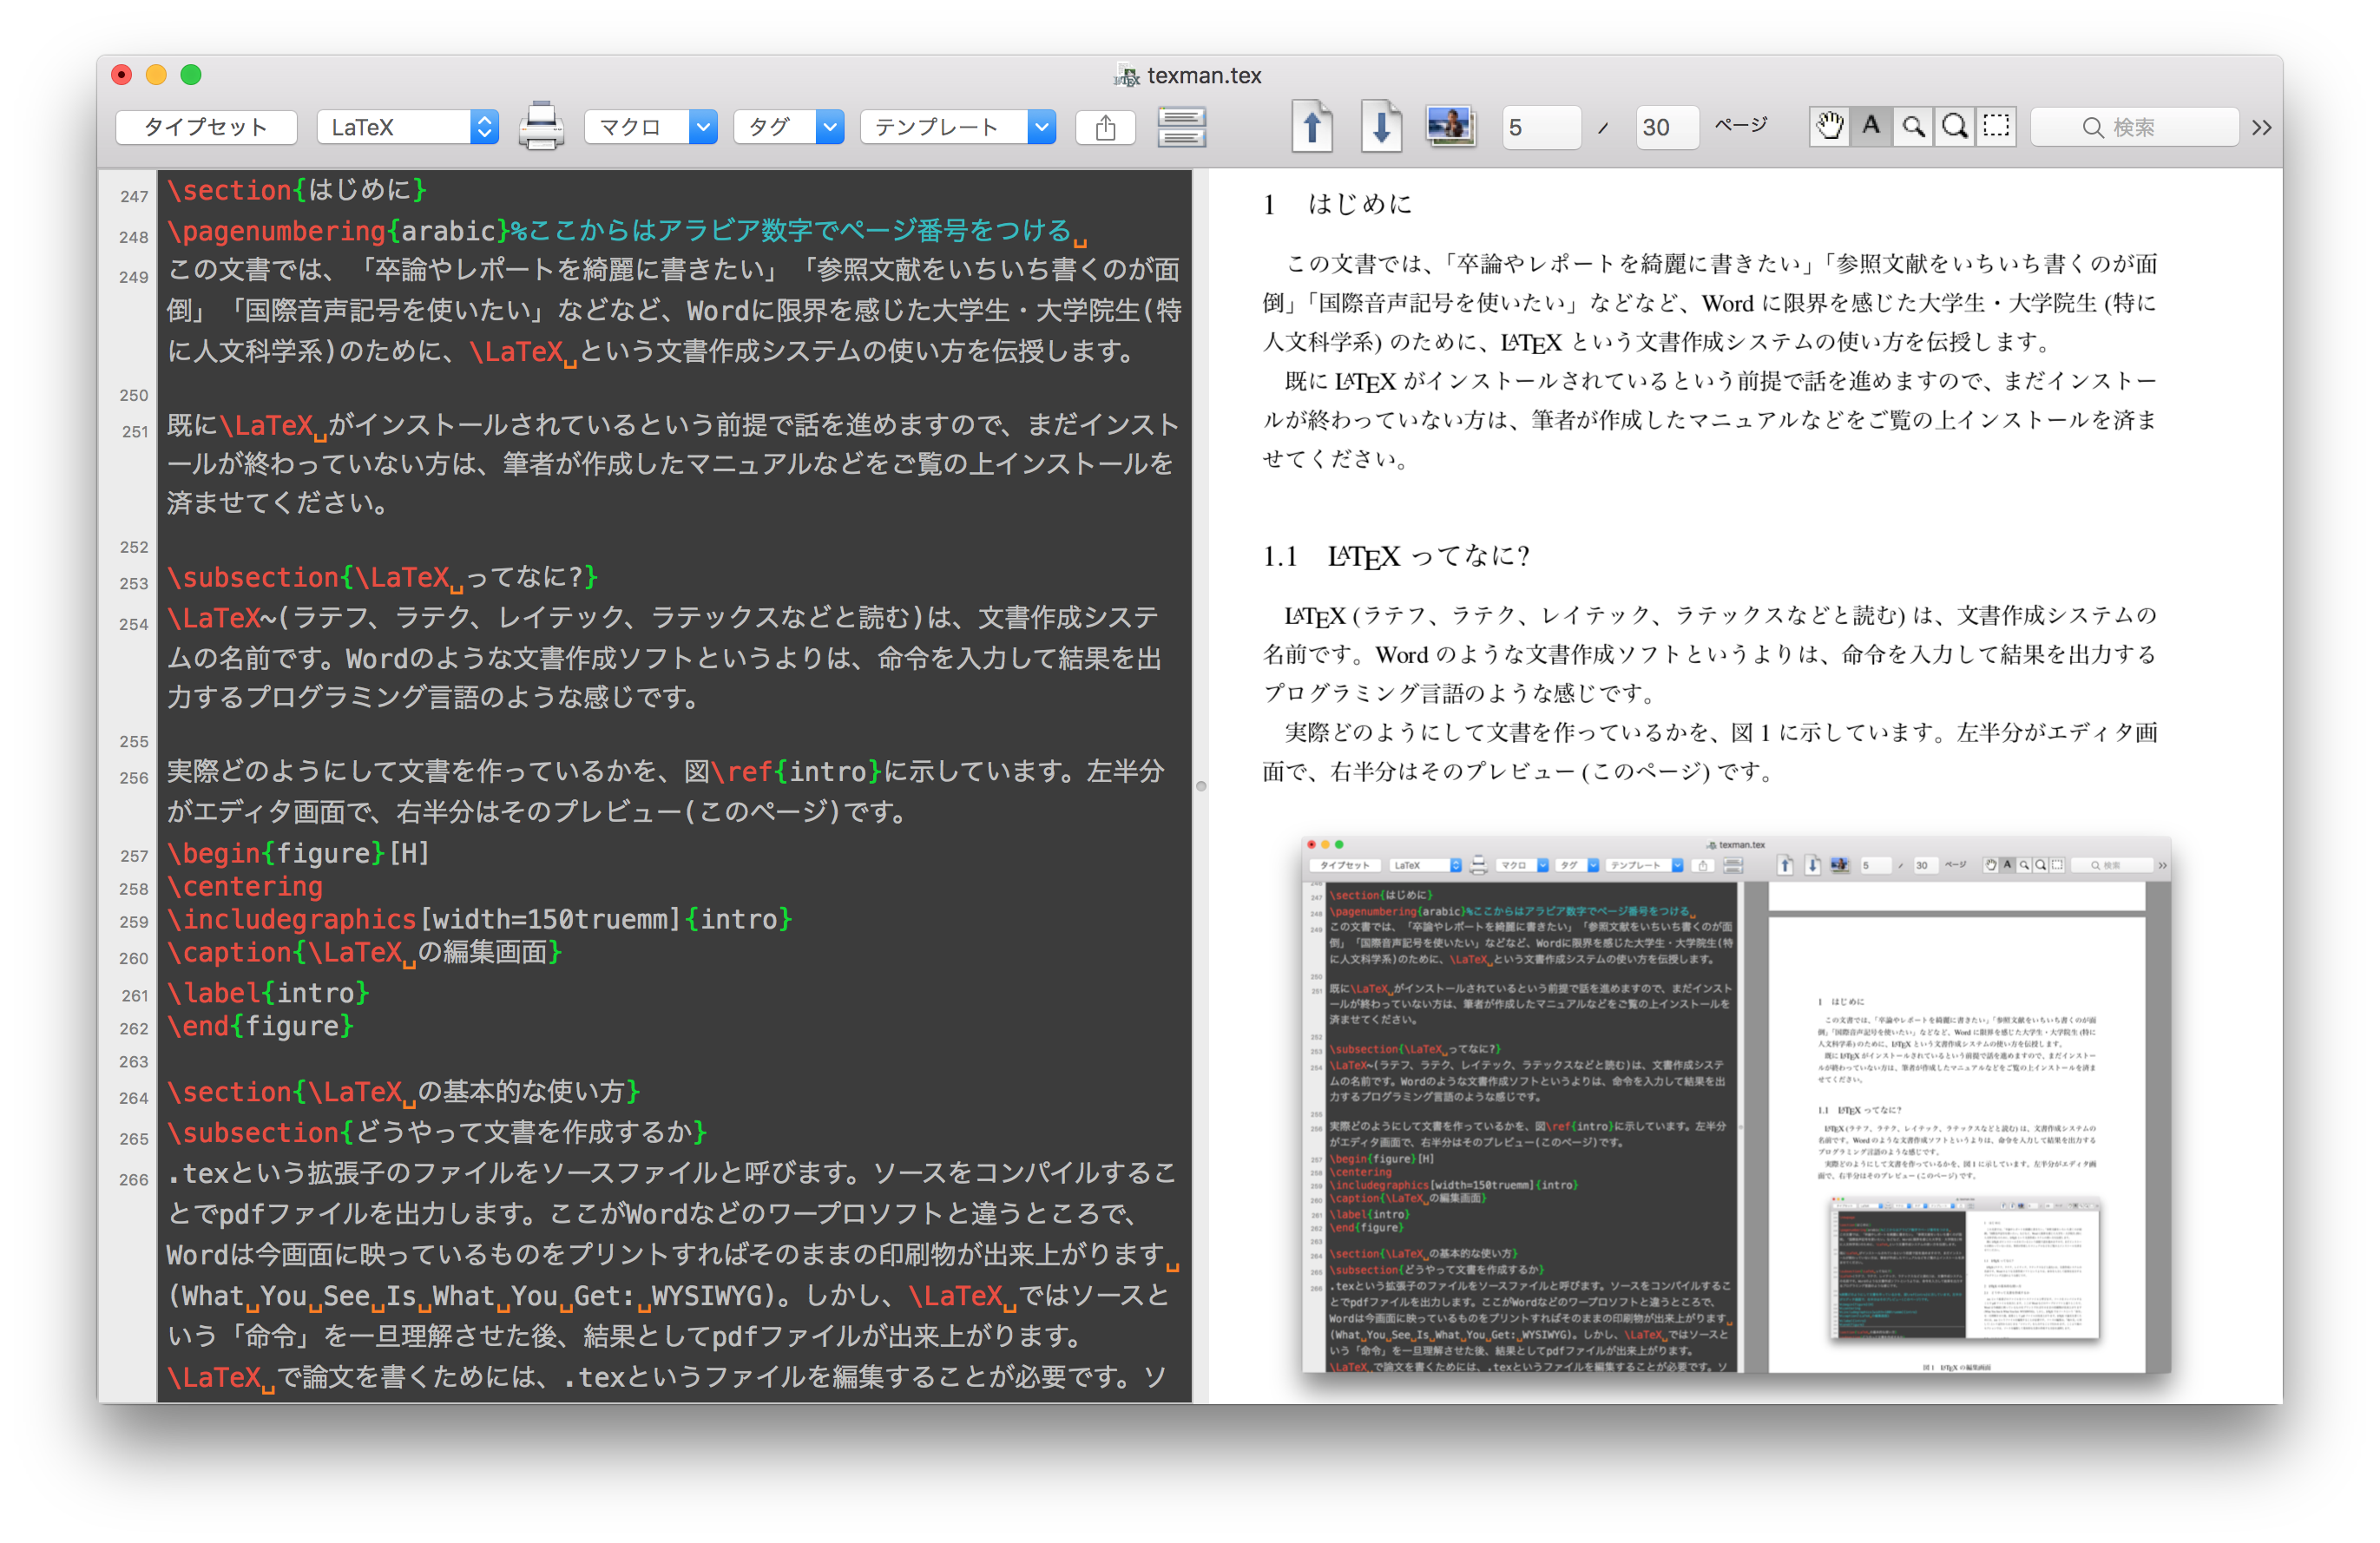
\includegraphics[width=150truemm]{intro}
\caption{\LaTeX の編集画面(MacOS)}
\label{intro}
\end{figure}
編集画面で打ち込んだ文字がそのまま印刷結果になるのではない、というところがWordなどのワープロソフトとの大きな違いです。自分が得たい出力結果を出すためには、このプログラミングのような書き方を覚えなければいけません。ちょっと敷居は高いですが、一緒に勉強していきましょう。

\subsection{\LaTeX を使うと何がいいの?}
\begin{screen}
\begin{enumerate}
\item 数式, 例文, 発音記号などの特殊な表記法が綺麗に出力できる
\item 参照文献の引用がとても楽
\item ユーザーによる拡張性が高い
\end{enumerate}
\end{screen}

\subsubsection{数式や例文が綺麗に出力できる}
\TeX~(\LaTeX の基になっているシステム)は、元々パソコンで数式を綺麗に出力できるように開発されました。なので、数式、あるいは言語学の例文のような「ちょっと特別な書き方が必要」な分野に関してはめっぽう強いです。ちょっと例を見てみましょう。

\begin{shadebox}
	\begin{equation}
		s^2 = 1/n\sum_{i=1}^n (x_i -\mu)^2
	\end{equation}


\ex
\begingl
\glpreamble Bzhedukh語の例文 \citep{payne1997}//
\gla \textipa{\v{c}Paalya-m} \textipa{\v{c}P@g\super wo-@r} \textipa{ya-\v{z}\super woa}//
\glb boy-\Erg{} filed-\Abs{} \Tsg{}-plows//
\glft `The boy plows field.'//
\endgl
\xe

\end{shadebox}
どうでしょう。Wordよりも綺麗に出力できているように見えませんか?

\subsubsection{参照文献の引用がとても楽}
文中で引用した全ての文献は、特定の形式に沿って参照文献として示さないといけません。「インデントするのが面倒くさい」「タイトル、巻号なんかを書く順番がわからない」などでお悩みではありませんか?\LaTeX ならそのお悩みは一発で解決できます。文中で文献を引用するだけで、自動的に参照文献一覧を作ってくれます。

\subsubsection{ユーザによる拡張性が高い}
Wordを使っていると、痒い所に手が届かなかったり、あるいは逆にどうでもいいところでお節介をされて困ることはありませんか? \LaTeX なら、全ての設定が全て自分でできます。

さあ、みなさんも\LaTeX を始めて見ませんか?

\section{\LaTeX の基本的な使い方}
\begin{tcolorbox}[colback=white,colframe=black,colbacktitle=mygreyl,coltitle=black,title=この章で説明すること]

\begin{itemize}[style=nextline]
\item エディタを立ち上げる
\item エディタを使って簡単な文書を生成する
\item 文字に装飾をする
\end{itemize}

\end{tcolorbox}


\subsection{エディタの使い方}
文書の編集を助けてくれるアプリケーションのことを「エディタ」と呼びます。エディタには、\TeX Worksや\TeX Shopなどがあります。まずは、エディタを立ち上げます。

\vspace{1ex}

\begin{description}[style=nextline]
\item [\textbf{Windowsユーザ}]「Windowsメニュー/すべてのプログラム/\TeX Live 2017」の中に\TeX Works Editorというアプリケーションがあるはずです。これを選択して立ち上げると、白紙の画面が出てきます。ここに命令を入力して文書を作ります。

\item [\textbf{Macユーザ}] アプリケーションフォルダに\TeX Shopというものが入っていると思います。これを選択して立ち上げると、白紙の画面が出てきます。ここに命令を入力して文書を作ります。
\end{description}

\subsection{簡単な文書を作ってみよう}
エディタを立ち上げたら、簡単な文書を作ってみましょう。

まずはじめに、\LaTeX で必ず行わなければいけないのが、(1)文書クラスの指定と(2)ドキュメント環境の作成です。
「新規作成」を行うと白紙の文書が作成できると思いますが、そこに
\begin{screen}
\begin{verbatim}
\documentclass[11pt]{jsarticle}
\begin{document}
aiueo
\end{document}
\end{verbatim}
\end{screen}
のように打ち込んでください。\verb|\|という文字(バックスラッシュ)は¥マークで代用しても構いません。打ち込んだら「タイプセット」をしてください。

\vspace{1ex}

\begin{tcolorbox}[colback=white,colframe=black,colbacktitle=mygreyl,coltitle=black,title=タイプセットの方法]

\begin{description}[style=nextline]
\item [\textbf{\TeX Worksユーザ}]左上に緑色の三角のボタンがあります。ボタンの右にあるプルダウンメニューに「pLaTeX(ptex2pdf)」と表示されていることを確認し、三角ボタンを押してください。Ctrl+Tでもタイプセットができます。

\item [\textbf{\TeX Shopユーザ}] 左上に「タイプセット」と書かれたボタンがあります。ボタンの右にあるプルダウンメニューに「LaTeX」と表示されていることを確認し、タイプセットボタンを押してください。command+Tでもタイプセットができます。
\end{description}

\end{tcolorbox}



タイプセットが成功すれば``aiueo''とだけ書かれた文書が出来るはずです。

ここで行っているのは、文書クラスの指定とドキュメント環境の作成です。まず、文書クラスの指定では「どんなスタイルの文書を作るか」を指定します。特に好みがなければ、jsarticleというクラスを指定しておくのがよいでしょう。ドキュメント環境とは\verb|\begin{document}|と\verb|\end{document}|で囲まれた部分のことです。ドキュメント環境を作るというのは「ここからここまでが作りたい文書です」という宣言をするということです。二つとも絶対に必要な手順なので、何も考えずに打ち込んでください。

\subsection{文字の処理}
\subsubsection{改行}
エディタ画面で以下のように入力をしても改行されません。\\
\begin{minipage}{1\textwidth}
\begin{tabular}{c c}
\begin{minipage}[h]{.5\textwidth}
\begin{screen}
\begin{verbatim}
入力:
いろはにほへと
ちりぬるを
\end{verbatim}
\end{screen}
\end{minipage}
&
\begin{minipage}[h]{.5\textwidth} 
\begin{shadebox}
出力:\\
いろはにほへと
ちりぬるを
\end{shadebox}
\end{minipage}
\end{tabular}
\end{minipage}\\

\noindent もし「いろはにほへと」と「ちりぬるを」の間で改行をしたいなら、\verb|\\|という記号を「いろはにほへと」の後にはさみます。\\
\begin{minipage}{1\textwidth}
\begin{tabular}{c c}
\begin{minipage}[h]{.5\textwidth}
\begin{screen}
\begin{verbatim}
入力:
いろはにほへと\\
ちりぬるを
\end{verbatim}
\end{screen}
\end{minipage}
&
\begin{minipage}[h]{.5\textwidth} 
\begin{shadebox}
出力:\\
いろはにほへと\\
ちりぬるを
\end{shadebox}
\end{minipage}
\end{tabular}
\end{minipage}\\


\subsubsection{段落}
この\verb|\\|を使った改行は、新しい段落を作りません。新しい段落を作りたい時、つまり「行頭の字下げ(インデント)を行いたい時」は、行と行の間に空白の行を挿入することで新しい段落が作れます。\\
\begin{minipage}{1\textwidth}
\begin{tabular}{l r}
\begin{minipage}[h]{.5\textwidth}
\begin{screen}
\begin{verbatim}
入力:
いろはにほへとちりぬるをわかよたれそつねならむ

うゐのおくやまけふこえて
\end{verbatim}
\end{screen}
\end{minipage}
&
\begin{minipage}[h]{.5\textwidth} 
\begin{shadebox}
出力:\\
いろはにほへとちりぬるをわかよたれそつねならむ

\quad うゐのおくやまけふこえて
\end{shadebox}
\end{minipage}
\end{tabular}
\end{minipage}\\


段落を変えたいだけでなく段落の間に空白を一行はさみたいときは、\verb|\bigskip|と入力します。\\
\begin{minipage}{1\textwidth}
\begin{tabular}{l r}
\begin{minipage}[h]{.5\textwidth}
\begin{screen}
\begin{verbatim}
入力:
いろはにほへとちりぬるをわかよたれそつねならむ
\bigskip

うゐのおくやまけふこえて
\end{verbatim}
\end{screen}
\end{minipage}
&
\begin{minipage}[h]{.5\textwidth} 
\begin{shadebox}
出力:\\
いろはにほへとちりぬるをわかよたれそつねならむ
\bigskip

\quad うゐのおくやまけふこえて
\end{shadebox}
\end{minipage}
\end{tabular}
\end{minipage}\\


一行空けたいけれどもインデントはしたくない、という場合は段落のはじめに\verb|\noindent|と入力します。\\
\begin{minipage}{1\textwidth}
\begin{tabular}{l r}
\begin{minipage}[h]{.55\textwidth}
\begin{screen}
\begin{verbatim}
入力:
いろはにほへとちりぬるをわかよたれそつねならむ
\bigskip

\noindent うゐのおくやまけふこえて
\end{verbatim}
\end{screen}
\end{minipage}
&
\begin{minipage}[h]{.45\textwidth} 
\begin{shadebox}
出力:\\
いろはにほへとちりぬるをわかよたれそつねならむ
\bigskip

うゐのおくやまけふこえて
\end{shadebox}
\end{minipage}
\end{tabular}
\end{minipage}\\

ここで気をつけてほしいのは、\verb|\noindent|と入力した後にそのまま文を続けず、必ず半角スペースを一つ挟むようにするということです。半角スペースをいれないで
\begin{screen}
\verb|\noindentうゐのおくやまけふこえて|
\end{screen}
のように入力すると、コンソール画面で``Undefined control sequence''というエラーが返ってきてタイプセットが失敗してしまいます。これは、\verb|\|からはじまる文字列が「コマンド」として認識されるために起こるエラーです。上の例で言えば「noindent」という命令を読み込ませたいところで、「noindentうゐのおくやまけふこえて」という命令をしてしまっているということです。しかし、「\verb|\noindent|うゐのおくやまけふこえて」というコマンドは定義されていませんので、「そんな命令しらない!」ということでエラーが返ってくるわけです。半角スペースを入力することで、「ここで命令は終わりです」ということを表します。\verb|\|noindent以外のコマンドでも、コマンドを入力し終わった後に文字を続けずに半角スペースを入力するよう気をつけてください。

このように、コマンドを書くのに失敗するとエラーが返ってきてしまいます。でも心配せずにコンソールに表示されたエラーをきちんと読んでください。エラーメッセージを読めば、何がダメだったのかは大体分かります。よくありがちなものとしては、括弧を閉じていない、コマンドのスペルミスをしている、コマンドのあとにそのまま文字入力を続けてしまっている、などがあります。

\subsubsection{空白}
\LaTeX では、空白の処理は少し複雑です。例えば、
\begin{screen}
入力: \verb*|い  ろ は   に|\\
出力: い  ろ は   に
\end{screen}
このように半角のスペースをいくつ重ねても全て半角のスペース一つ分として処理されてしまいます。そこで、半角スペースを続けたい時には\verb|~|という記号を使います。
\begin{screen}
入力: \verb*|い~~~~ろ~は~~~~~~~~に|\\
出力: い~~~~ろ~は~~~~~~~~に
\end{screen}
このように、半角スペースを複数重ねることができます。なお、全角スペースの場合は重ねたら重ねた分だけ処理されますので、心配はいりません。

\subsection{文字の装飾}\label{adorn}
ここまででは「地の文」をどう入力するかを説明しました。このセクションでは、「地の文」に装飾をつける方法を説明していきます。

今までの部分で、\verb|\|から始まっている部分がありました。これを「コマンド」と呼び、コンピュータに与える命令を記述します。例えば、Hello World!という文字列をイタリックにしたいとしましょう。その時は以下のような記述をします。
\begin{screen}
入力: \verb|\textit{Hello World!}|\\
出力: \textit{Hello World!}
\end{screen}
この入力の意味を解説します。\verb|\textit|というのは「コマンド」で、ある操作をコンピュータに命令します。\verb|\textit|というのは、「\verb|{}|で囲った部分をイタリックにせよ」という命令です。同様のコマンドとして、文字列を太字にする\verb|\textbf|などがあります。表\ref{adorn}は、文字の装飾コマンドをまとめたものです。和文フォントは3つ、欧文フォントは7つの命令がありますので、これらを組み合わせて使ってください。

\begin{table}[h]
\centering
\caption{文字に装飾を加えるコマンド}
\label{adornchart}
\begin{tabular}{|l|lc|} \hline
\small
\multirow{5}{*}{\footnotesize 和文} & \verb|\textmc{}| & \textmc{細明朝体} \\
& \verb|\textmc{\textbf{}}| & \textmc{\textbf{太明朝体}} \\
& \verb|\textgt{}| & \textgt{細ゴシック体} \\
& \verb|\textgt{\textbf{}}| & \textgt{\textbf{太ゴシック体}} \\
%& \verb|\textmg{}| & \textmg{丸ゴシック体} \\ \hline
\multirow{11}{*}{\footnotesize 欧文}  & \verb|\textrm{}| &\textrm{Roman(ウロコ付き)} \\
& \verb|\textbf{}| & \textbf{Boldface(ウロコ付き太字)} \\
& \verb|\textit{}| & \textit{Italic(イタリック)} \\
& \verb|\textit{\textbf{}}| & \textit{\textbf{Bold Italic(イタリック太字)}} \\
& \verb|\textsl{}| & \textsl{Slanted(斜字体)} \\
& \verb|\textsl{\textbf{}}| & \textsl{\textbf{Slanted(斜字体太字)}} \\
& \verb|\textsc{}| & \textsc{Small Caps(スモールキャピタル)} \\
& \verb|\textsc{\textbf{}}| & \textsc{\textbf{Bold SC(スモールキャピタル太字)}} \\
& \verb|\textsf{}| & \textsf{Sans Serif(ウロコなし)} \\
& \verb|\textsf{\textbf{}}| & \textsf{\textbf{Bold Sf(ウロコなし太字)}} \\
& \verb|\texttt{}| & \texttt{Typewriter(計算機)} \\
& \verb|\texttt{\textbf{}}| & \texttt{\textbf{Typewriter(計算機太字)}} \\ \hline
\end{tabular}
\end{table}

\noindent 表\ref{adornchart}で示した字体以外は\textgt{\textbf{基本的に使うことができません。}}

\LaTeX では、フォントサイズの指定もコマンドで行います。サイズ指定には、基本サイズからの縮小率を指定する「相対指定」と、変更後のサイズをそのまま指定する「絶対指定」を行います。

\begin{table}[H]
\centering
\caption{文字の大きさを指定するコマンド}
\label{fontchart}
\begin{tabular}{|l|l|c|} \hline
\multicolumn{2}{|l|}{入力} & 出力 \\ \hline
\multirow{10}{*}{相対} & \verb|{\tiny M}| & {\tiny M} \\
& \verb|{\scriptsize M}| & {\scriptsize M} \\
& \verb|{\footnotesize M}| & {\footnotesize M} \\
& \verb|{\small M}| & {\small M} \\
& \verb|{\normalsize M}| & {\normalsize M} \\
& \verb|{\large M}| & {\large M} \\
& \verb|{\Large M}| & {\Large M} \\
& \verb|{\LARGE M}| & {\LARGE M} \\
& \verb|{\huge M}| & {\huge M} \\
& \verb|{\HUGE M}| & {\HUGE M} \\ \hline
\multirow{3}{*}{絶対}& \verb|{\fontsize{11pt}{11pt}\selectfont M}| & {\fontsize{11pt}{11pt}\selectfont M} \\
& \verb|{\fontsize{4.235truemm}{4.235truemm}\selectfont M}| & {\fontsize{4.235truemm}{4.235truemm}\selectfont M} \\
& \verb|{\fontsize{8truemm}{8truemm}\selectfont M}| & {\fontsize{8truemm}{8truemm}\selectfont M} \\ \hline

\end{tabular}
\end{table}

\verb|\large|や\verb|\small|というコマンドは、それぞれ「基本のフォントサイズ(11pt)から〇〇倍する」という相対指定コマンドです。\verb|\fontsize|というのは絶対指定ですが、後の方に\verb|\selectfont|というよくわからないコマンドがくっついています。これは文字送りを指定するコマンドですが、あまり気にしなくてよいです。

このように、色々なコマンドを使って文字の装飾を行っていきます。他にも上付き、下付き、下線、ダイアクリティカルマークの入力などの装飾も全てコマンドで行います。文字の装飾に限らず様々なコマンドの説明があるので、\href{http://www.latex-cmd.com/}{LaTeXコマンド集}というサイトを是非参照してみてください



\subsection{章立て}
まとまった形式の文書を書くときには、章立てが必要になってきます。具体的な使い方を見ていきましょう。

\verb|\section|というコマンドを入力することで、そこにあらたな節を作ります。

\bigskip
\begin{minipage}{1\textwidth}
\begin{tabular}{l r}
\begin{minipage}[h]{.5\textwidth}
\begin{screen}
\begin{verbatim}
入力: \section{ほげほげ}
\end{verbatim}
\end{screen}
\end{minipage}
&
\begin{minipage}[h]{.5\textwidth} 
\begin{shadebox}
出力: \section{ほげほげ}

\end{shadebox}
\end{minipage}
\end{tabular}
\end{minipage}\\

\verb|\section{}|という命令の解説をしましょう。これは、「\verb|{}|で囲った部分をタイトルとする新しい節を作れ」という命令で、\LaTeX が自動的に節番号も振ってくれます。この文書では既にsectionが二つありますので、ここで新たにsectionを指定したことで自動的に「3」という番号を振ってくれたわけです。文字の大きさ、太さ、フォントや前後の空白も自動で設定してくれます。subsection以下についても同様に処理してください。
\setcounter{section}{2} %さっきのsectionの説明で余計なsectionを作ってしまったので、ここでカウンタをリセットしています。

\section{スタイルファイル(拡張パッケージ)の導入}\label{sty}
参照文献のセクションでも少し触れましたが、\LaTeX では機能を拡張するためにスタイルファイルというものを導入することができます。スタイルファイルの拡張子はstyです。スタイルファイルの中には、\LaTeX のインストールと同時にダウンロードされるものもあれば、自分でダウンロードしてこなければいけないものもあります。ここでは、スタイルファイルの導入の仕方を説明します。

\subsection{あらかじめダウンロードされているものの導入}
前のセクションで使用したnatbib.styは、大方の場合あらかじめパソコンの中に入っています。このようなスタイルファイルの場合、前のセクションで行ったように、\verb|\documentclass{}|と\verb|\begin{document}|の間に\verb|\usepackage{(ファイル名)}|と指定することで導入できます。

\subsection{まだパソコンに入っていないものの導入}
\href{https://www.ctan.org/pkg}{CTAN}というサイトではスタイルファイルが多数配布されています。ここでは、natbib.styというスタイルファイル(次の「参照文献の引用」セクションでもつかいます)を導入してみましょう。まず\href{https://www.ctan.org/pkg}{CTAN}にアクセスし、検索フォームからnatbibと検索してください。検索結果のどこかに「Package natbib」というリンクがあるはずなので、そこをクリックしてください。natbibのページに移行したら、Downloadと書かれたリンクがあります。そこをクリックして、zipファイルをダウンロードして解凍してください。

ここから.styファイルを生成する作業に入ります。まず、コマンドラインのアプリケーション(Winならコマンドプロンプト、Macならターミナル)を立ち上げてください。コマンドラインから、解凍したnatbibというフォルダの中に移動してください。例えば、/Users/staff/Downloads/natbibというパスに当該ファイルがあるなら、コマンドラインで\verb|cd /Users/staff/Downloads/natbib|と移動してください。移動が完了したら、コマンドラインで \verb|latex natbib.ins|と入力してください。そうすると、natbib.styというファイルが生成されているはずです。このnatbib.styを編集中の.texファイルと同じディレクトリに置いてください。

次に、生成したnatbib.styを文書に導入します。文書内で、文書クラスの指定(\verb|\documentclass{}|という部分)と\verb|\begin{document}|の間に、\verb|\usepackage{natbib}|と記入してください。

これで新しいスタイルファイルの導入が完了しました。これ以降は文書内でnatbibで拡張された機能を使うことができます。どのようにその機能を使うかは次節以降をご覧ください。

\section{論文で使うあれこれ}
さて、ここまでで基本的な文書の作り方を解説してきました。ここからは、基本的な論文で使う色々なものの挿入の仕方について説明していきたいと思います。

\subsection{表の挿入}\label{chartins}
表の挿入の仕方を見ていきます。
\subsubsection{普通の表}
以下のように入力すると、
\begin{screen}
\footnotesize
\begin{verbatim}
\begin{table}[h]
\centering
\caption{変化表}
\label{amicus}
\begin{tabular}{|l|c|c|c|c|c|c|} \hline
	  & 主格 & 呼格 & 属格 & 与格 & 対格 & 奪格 \\ \hline
	単数 & amicus & amice & amici & amico & amicum & amico \\ \hline
	複数 & amici & amici & amicorum & amicis & amicos & amicis \\ \hline
\end{tabular}
\end{table}
\end{verbatim}
\end{screen}

\begin{table}[h]
\centering
\caption{変化表}
\label{amicus}
\begin{tabular}{|l|c|c|c|c|c|r|} \hline
	  & 主格 & 呼格 & 属格 & 与格 & 対格 & 奪格 \\ \hline
	単数 & amicus & amice & amici & amico & amicum & amico \\ \hline
	複数 & amici & amici & amicorum & amicis & amicos & amicis \\ \hline
\end{tabular}
\end{table}

このように出力されます。コマンドの意味を確認して行きましょう。
\begin{itemize}
\item まず、全体をtable環境で囲みます。

\item 一行目のhという部分は「この場所に出力せよ」という意味です。

\item 二行目の\verb|\|centeringというのは、「表全体を中央揃えにせよ」という意味です。これを入力しないと左寄せになります。

\item 三行目の\verb|\|captionというのは、表の上に表示される名前です。

\item 四行目の\verb|\|labelというのは、また後で説明しますが、この表の番号を参照する時に使います。このlabelはオプションなので、入力しなくても良いです。
\item
tabular環境で囲まれている部分が表の本体になります。
\begin{verbatim}
{|l|c|c|c|c|c|}
\end{verbatim}
というのは、縦の罫線と各セル内での文字の位置を設定している箇所です。\verb~|~でどこに罫線を引くかを決定し、lとcとrで「列の数」と「各セル内での文字の位置」を決定します。lなら左寄せ、cなら中央揃え、rなら右寄せです。
\begin{verbatim}
{|lcccc|}
\end{verbatim}
例えば、以上のように記述すると、5列で左端と右端にだけ縦罫線を引くという指定になります。

\item \verb|\\ \hline|というのは、「行の下側に横罫線を引き、ここでこの行は終われ」という意味です。\verb|\\|を入力しないとコンパイルエラーになりますので、行の終わりには必ず入力してください。

\item 6行目から8行目からは各セルの内容です。セル同士は\&で区切ってください。空白にするセルがあれば、何も入力しないまま\& を入力してください。\& の数と列数が合わない場合コンパイルエラーになります。
\end{itemize}

\subsubsection{セルの結合}
セルを結合させたい場合は、横に結合する場合\verb|\multicolumn{}{}{}|、縦の場合\verb|\multirow{}{}{}|を使います。

\bigskip
\begin{screen}
\footnotesize
\begin{verbatim}
\begin{table}[h]
\centering
\caption{横結合セル}
\label{amicus}
\begin{tabular}{|l|c|c|} \hline
		\multicolumn{3}{|c|}{A} \\ \hline
		\multicolumn{2}{|c|}{B} & C \\ \hline
		D & E & F \\ \hline
\end{tabular}
\end{table}
\end{verbatim}
\end{screen}

\begin{table}[h]
\centering
\caption{横結合セル}
\label{multicolumn}
\begin{tabular}{|l|c|c|} \hline
		\multicolumn{3}{|c|}{A} \\ \hline
		\multicolumn{2}{|c|}{B} & C \\ \hline
		D & E & F \\ \hline
\end{tabular}
\end{table}

\verb|\multicolumn{}{}{}|の引数は、一番目から順に「横に結合するセルの数」、「セル内の文字の位置と罫線」、「セルの内容」です。

\bigskip
\begin{screen}
\footnotesize
\begin{verbatim}
\begin{table}[h]
\centering
\caption{縦結合セル}
\label{multirow}
\begin{tabular}{|l|c|c|} \hline
		\multirow{3}{*}{A} & \multirow{2}{*}{B} & C \\ \cline{3-3}
		& & D \\ \cline{2-3}
		 & E & F \\ \hline
\end{tabular}
\end{table}
\end{verbatim}
\end{screen}

\begin{table}[h]
\centering
\caption{縦結合セル}
\label{multirow}
\begin{tabular}{|l|c|c|} \hline
		\multirow{3}{*}{A} & \multirow{2}{*}{B} & C \\ \cline{3-3}
		& & D \\ \cline{2-3}
		 & E & F \\ \hline
\end{tabular}
\end{table}

\verb|\multicolumn{}{}{}|の引数は、順番に「縦に結合するセルの数」、「列の位置(通常は*でよい)」、「セルの内容」です。結合されたことで入力の必要が無くなったセルは空白にしておいてください。\verb|\cline{}|の括弧の中身は、「罫線を引き始めるセル-引き終わるセル」で指定してください。

以上が表の組み方です。
\subsection{図の挿入}\label{figins}
図を挿入するにはfigure環境と\verb|\includegraphics|を使います。挿入したい画像は、.texが入っているフォルダと同じディレクトリに入れておくようにしてください。

\bigskip
\begin{screen}
\begin{verbatim}
\begin{figure}[h]
\caption{肝臓}
\centering

\includegraphics[width=50truemm]{liver}
\label{liver}
\end{figure}
\end{verbatim}
\end{screen}

\bigskip
\begin{figure}[h]
\caption{肝臓}
\centering

\includegraphics[width=50truemm]{liver}
\label{liver}
\end{figure}

\bigskip
\verb|\caption{}|と\verb|\label{}|は表の挿入の時と同じです。width=では、挿入する画像の横幅がどれくらいの長さになるかを指定します。\verb|\includegraphics{}|の括弧の中には、挿入する画像のファイル名の拡張子を外した部分を書いてください。

\subsection{相互参照}\label{sansyoo}
さて、ここまでで表や図を挿入する方法を見てきました。論文中では、これらの図に言及して、「表\ref{multirow}を見ると…」などと書くことがあるでしょう。その時はいちいち表の番号を手打ちしてもよいですが、途中に別の表を挿入したりすると表番号が変わってしまい、いちいち修正するはめになります。それを防ぐために活躍するのが「相互参照」という機能です。

今まで作って来た図表では、\verb|\label{}|というコマンドを書いていたと思いますが、これはこの相互参照の時に活躍します。例えば、表\ref{multirow}の「縦結合セル」では\verb|\label{multirow}|というラベルを振っています。``multirow''というのがこの表の「名前」になるわけです。この表の番号を参照したければ、\verb|\ref{}|というコマンドを使って以下のように記述します。

\bigskip
\begin{minipage}{1\textwidth}
\begin{tabular}{l r}
\begin{minipage}[h]{.5\textwidth}
\begin{screen}
\begin{verbatim}
入力: 表\ref{multirow}によると
\end{verbatim}
\end{screen}
\end{minipage}
&
\begin{minipage}[h]{.5\textwidth} 
\begin{shadebox}
出力: 表\ref{multirow}によると

\end{shadebox}
\end{minipage}
\end{tabular}
\end{minipage}\\

\verb|\ref{}|で参照してくれるのは番号の数字だけなので、「表」とか「図」とかいった部分は自分で入力してください。

また、\verb|\ref{}|で参照できるのは図や表だけではありません。節や頁など、あらゆるものを参照することができます。例えば、この文書ではセクション\ref{figins}に\verb|\label{figins}|というラベルを振っています。これを利用して以下のように記述できます。

\bigskip
\begin{minipage}{1\textwidth}
\begin{tabular}{l r}
\begin{minipage}[h]{.5\textwidth}
\begin{screen}
\begin{verbatim}
入力: \ref{figins}節を参照
\end{verbatim}
\end{screen}
\end{minipage}
&
\begin{minipage}[h]{.5\textwidth} 
\begin{shadebox}
出力: \ref{figins}節を参照

\end{shadebox}
\end{minipage}
\end{tabular}
\end{minipage}\\

\subsection{脚注の挿入}
\LaTeX で文書に脚注を挿入するためには、\verb|\footnote{}|というコマンドを使います\footnote{ここで示した例は特殊な環境で使っているため番号表示がアルファベットになっていますが、通常に使った場合このように数字表記になります}。脚注を付けたい直後の箇所でコマンドを使い、括弧の中に注の内容を書き込みます。

\bigskip
\begin{minipage}{1\textwidth}
\begin{tabular}{l r}
\begin{minipage}[h]{.5\textwidth}
\begin{screen}
\footnotesize
\begin{verbatim}
ダース・ヴェイダーはシス\footnote{ダークサイドのフォースを信奉する集団}の暗黒卿である
\end{verbatim}
\end{screen}
\end{minipage}
&
\begin{minipage}[h]{.5\textwidth} 
\begin{shadebox}
ダース・ヴェイダーはシス\footnote{ダークサイドのフォースを信奉する集団}の暗黒卿である

\end{shadebox}
\end{minipage}
\end{tabular}
\end{minipage}\\

\section{参照文献の引用}
\subsection{BiBTeXの使い方}
\begin{screen}
\begin{enumerate}
\item 書誌情報が入力されたファイルを作る
\item 入力した書誌情報を文中で引用する
\item 引用スタイルを指定する
\item 文中で書誌情報を入力したファイルを指定する
\item タイプセットする
\item 参照文献リストが作成される
\end{enumerate}
\end{screen}

\LaTeX で参照文献を引用するには、ちょっとした手間が必要です。最初に「参照文献リストを作るのがWordに比べて楽」と言ったじゃないか、と思うかもしれませんが、正確にいうと「最初はちょっと手間がかかるが、一回設定してしまえばあとは楽」という意味です。上に書いたステップごとに進んで行きましょう。なお、まだ前セクションの「スタイルファイルを導入する」をご覧になっていないかたは、そちらをご覧になってからもう一度ここに戻ってきてください。

\subsection{書誌情報を入力する}
\LaTeX で文献を引用するためには、まず書誌情報がつまったファイルを作成する必要があります。ファイルの作成には、エディタとは別のアプリケーションを使います。MacならBiBDeskというアプリケーションが同時にインストールされているので、それを使ってください。他のOSなら、JabRefというJavaアプリがどのOSでも使えるはずなので、それをインストールしてください。自分のお好みのもの(Mendeley, Zoteroなど)がある方はそれで結構です。

これらのアプリケーションを立ち上げ、新しいファイルを作成してください。BibDeskなら、File$\rightarrow$Newb Bibliography を押してください。 JabRefなら、左上の``New BibTeX database''というボタン(白ヌキの紙のようなアイコン)を押してください。

それでは、お手元にある適当な本の書誌情報を入力してみてください。BiBDeskなら上の方にある緑色の+ボタンを押し、JabRefなら上の方にある白抜きの+ボタンを押します。JabRefであれば、最初に「エントリータイプを入力する」画面が出ます。これは、これから入力するものがどんな種類の本なのかを決定する場面です。本の種類によって引用の仕方が変わります(例えば、収録されている論集の名前を入力する必要があるかどうか、など)ので、最適なものを選ぶようにしてください。後から変更もできますので、分からない時はとりあえずbookかarticleを選択しておきましょう。BiBDeskではこの画面は表示されませんが、右上にデフォルトではbookと表示されている欄がありますので、そこで最適なものを選んでください。

書誌情報に入力する情報には、「required field」と「optional field」と「cite-key(BiBtex-key)」の3種類があります。required fieldとは、必ず入力しなければいけないもの(著者名、タイトルなど)です。optional fieldとは、入力しなくてもよいもの(発行月や出版地など)です。cite-keyは半角英数ならなんでもよいのですが、自分が後で分かりやすくなるような名前を付けておきましょう。私はいつも「名字 年」という形式にしています。書誌情報を入力する際に絶対に気をつけて欲しいのが以下の3点です。
\begin{enumerate}
\item\textbf{\large 日本語文献の場合、必ずYomiフィールドに著者の読みを\textcolor{magenta}{名姓の順で}記入すること}。これを入力しないと、参考文献リストが名前順に表示されなくなりますので、気をつけてください。
\item 漢字の著者を入力する時には\textbf{\large \textcolor{magenta}{姓名の順で}苗字と名前の間に半角スペースを入れること}を注意してください。こうしないと苗字と名前が一つながりの名前として認識されます。
\item \textbf{\large cite-key(BiBtex-key)を必ず入力すること。}これを入力しないと、文書中で引用することができません。
\end{enumerate}

書誌情報の入力が終わったら、編集中の.texファイルがあるのと同じディレクトリに.bibファイルを保存してください。この時、.bibファイルの名前はまた後で使いますので、わかりやすいものにしておいてください。

\subsection{引用する}
BiBTeXで書誌情報の入力が終わったら、そこで入力したcite-keyを使って引用していきます。
\bigskip

\begin{table}[H]
\caption{citation}
\centering
\begin{tabular}{cc}\toprule
\verb|\citet{jakobson1963}| & \citet{jakobson1963} \\
\verb|\citep{jakobson1963}| & \citep{jakobson1963} \\
\verb|\citet[cf.][12]{jakobson1963}| & \citet[cf.][12]{jakobson1963} \\
\verb|\citealp{jakobson1963}| & \citealp{jakobson1963} \\
\end{tabular}
\label{default}
\end{table}%
{\footnotesize
\begin{screen}
\begin{verbatim}
\citet{sakuma1941}, \citet{hattori1976},
\citet{postal1970}, \citet{paul1978},
\citet{aikhenvald2006}, \citet{kindaichi1955},
\citep{ueno1997}, \citep{kiparsky1968},
\citep{shibatani1978}, \citep{haegeman1994},
\citep{jakobson1963}, \citep{haegeman1994},
\citep[.cf][112]{nansei2005}, \citet[][12]{urabe2016}
\end{verbatim}
\end{screen}\\

\begin{shadebox}
\citet{sakuma1941}, \citet{hattori1976},
\citet{postal1970}, \citet{paul1978},
\citet{aikhenvald2006}, \citet{kindaichi1955},
\citep{ueno1997}, \citep{kiparsky1968},
\citep{shibatani1978}, \citep{haegeman1994},
\citep{jakobson1963}, \citep{haegeman1994},
\citep[.cf][112]{nansei2005}, \citet[][12]{urabe2016}
\end{shadebox}
}

\bigskip
\verb|\citet{}|は、発行年のみを括弧で囲うコマンドです。\verb|\citep{}|は、著者と発行年を括弧で囲うコマンドです。コマンドの後の最初の引数は、``see''や``.cf''などを入れるためのオプションです。二つ目の引数はページ数を指定したい時のオプションです。

\subsection{引用スタイルを指定する}
文献を引用スタイルには、分野、雑誌などの違いによって多岐に渡ります。ここでは、言語学、社会学、経済学などの理系寄りの人文系で標準的なスタイルを入力する方法を紹介します。つまり、文中の引用は 姓(発行年), 参照文献リストは 姓 名 (発行年) 「論文のタイトル」 『収録されている書籍, 雑誌のタイトル(あれば)』, 巻号, ページ, 出版社という形です。

\subsubsection{natbib.styを導入する}
科学系の論文の引用スタイルを導入するために、natbib.styを導入します。

文書クラスの指定(\verb|\documentclass{}|という部分)と\verb|\begin{document}|の間に、\verb|\usepackage{natbib}|と記入してください。

\subsubsection{jecon.bstを導入する}
natbib.styだけでは、日本語の文献に対応しません。そこで、武田史郎先生が作成した``jecon.bst''を導入します。

武田史郎先生のウェブサイト、「\href{http://shirotakeda.org/ja/tex-ja/jecon-ja.html#_3}{jecon.bst: 経済学用BibTeXスタイルファイル}」から、「ダウンロード」のページに行って、jecon.bstの最新版をダウンロードしてください。ダウンロードしたzipファイルを解凍すると、中に``jecon.bst''というファイルがあります。それを、編集中の.texファイルと同じディレクトリにいれてください。

ファイルの移動が終わったら、文書の\verb|\begin{document}|の後に、\verb|\bibliographystyle{jecon}|と記入してください。

\subsection{書誌情報が入ったファイルを指定する}
参照文献リストを挿入したい場所に\verb|\bibliography{(自分が入力した.bibファイルの名前)}|と入力してください

\subsection{タイプセットする}
参照文献リストを表示するためには、ちょっとしたタイプセットの手間が必要です。ここまできたらあと少しなので、頑張ってください。

まず、タイプセットボタンの横のプルダウンメニューに「LaTeX」(TeXWorksの場合はpLaTeX(ptex2pdf))と表示された状態で一回タイプセットを行ってください。その次に、プルダウンメニューから「BibTeX」(TeXWorksの場合はpBibTeX)と書かれたものを選択して、一回タイプセットボタンを押してください。その後、プルダウンメニューからLaTeXを再度選択し、あと二回タイプセットを行ってください。つまり、「LaTeX$\rightarrow$(p)BibTeX$\rightarrow$LaTeX$\rightarrow$LaTeX」と計四回タイプセットを行ってください。これで、参照文献リストが表示されます。

サイトコマンドで引用した文献は全て自動的に「参考文献」に載せられます。記載は引用した順番ではなく、著者の姓のアルファベット順です。同じ著者の文献が複数引用されている場合、発行年が古い順に載せられます。

\subsection{文献引用のまとめ}
まず、ファイル構成が以下のようになっているか確認してください。
\begin{screen}
\dirtree{%
.1 (適当なフォルダ).
.2 aiueo.tex (編集中のソースファイル).
.2 shoshi.bib (書誌情報を書いたファイル).
.2 jecon.bst (日本語文献の引用スタイルを指定するためのファイル).
}
\end{screen}
\vspace{1ex}

次に、文書の中身が以下のようになっているか確認してください。

\begin{screen}
\begin{verbatim}
\documentclass{jsarticle} %文書クラスの指定
\usepackage{natbib} %natbib.styの導入

\begin{document} 

\bibliographystyle{jecon} %jecon.bstの導入
\cite{payne1997} %ここに入力するのは自分が入力したcite-keyです
\bibliography{shoshi} %書誌ファイルの指定

\end{document}
\end{verbatim}
\end{screen}

次に、「LaTeX$\rightarrow$BibTeX$\rightarrow$LaTeX$\rightarrow$LaTeX」の順番でタイプセットを行ってください。

これで参照文献リストが作成できるはずです。これでもダメな場合、以下のことをためしてみてください。
\begin{enumerate}
\item 作業ファイル(フォルダの中にある、.tex, .bib, .bst以外の全てのファイル。例えば、.aux, .bbl, .blg, .log, .out, .pdf, .synctex.gzなど)を削除する
\item cite-keyを正しく入力しているか確認する。特に、大文字小文字に気を付けてください。
\end{enumerate}


\section{言語学用の設定}
\subsection{例文の挿入}

例文の挿入を補助するスタイルファイルはいくつかありますが、ここではexpex.styを紹介します。expex.styの詳しい使い方は、\href{https://ftp.kddilabs.jp/CTAN/macros/generic/expex/expex-doc.pdf}{ExPexのドキュメント}を参照してください。

\ex
hoge
\xe

\verb|\ex|と\verb|\xe|で囲った中に、始まる例文を入れます。すると、例文番号が自動でつきます。

\begin{screen}
\begin{verbatim}
入力:
\ex
arma virumque cano
\xe
\end{verbatim}
\end{screen}

\begin{shadebox}
出力:
\ex
arma virumque cano
\xe
\end{shadebox}

\bigskip
丸括弧の下にa, b...と続ける場合、\verb|\pex|と\verb|\xe|の間に\verb|\a|から例文を始めます。

\begin{screen}
\begin{verbatim}
入力:
\pex
    \a Graecia capta ferum victorem cepit
    \a tu fui ego eris
\xe
\end{verbatim}
\end{screen}

\begin{shadebox}
出力:

\pex
    \a Graecia capta ferum victorem cepit
    \a tu fui ego eris
\xe
\end{shadebox}

\bigskip

インターリニアーグロスを表示する場合、\verb|\ex|または\verb|\pex|の\verb|\xe|の間に、\verb|\begingl|と\verb|\endgl|を書き、その中に\verb|\glpreamble|, \verb|\gla|,\verb|\glb|, \verb|\glc|, \verb|\glft|という要素を入れます。\verb|\glpreamble|は例文の上につける説明文(省略可)、\verb|\gla|はグロスの1段目、\verb|\glb|はグロスの2段目、\verb|\glc|はグロスの3段目(省略可)、\verb|\glft|は訳文です。各要素の最後には//をつけます。

\begin{screen}
\begin{verbatim}
入力:
\ex
\begingl
\glpreamble 糸満方言の例文//
\gla uree namaa neen//
\glb uri=ja nama=ja nee-n//
\glc それ=\Top{} 今=\Top{} ない-\Ind{}//
\glft 「それは今はない」//
\endgl
\xe
\end{verbatim}
\end{screen}

\bigskip

\begin{shadebox}
出力:
\ex
\begingl
\glpreamble 糸満方言の例文//
\gla uree namaa neen//
\glb uri=ja nama=ja nee-n//
\glc それ=\Top{} 今=\Top{} ない-\Ind{}//
\glft 「それは今はない」//
\endgl
\xe
\end{shadebox}


\subsection{樹形図の挿入}
樹形図の挿入を行うにはいくつか方法があります。一つは、上山先生のサイトで配布されているTreeDrawerで樹形図を書いた後、スクリーンショットを取って図として挿入する方法です。これが余計なことをせず、ソースと格闘する必要もないかと思うのでオススメです。図の挿入は\ref{figins}を参照してください。TreeDrawerのインストールと使用方法は\href{http://www.gges.org/ueyama/TreeDrawer.shtml}{上山先生のサイト}を見てください。

他には、\LaTeX でスタイルファイルをインストールして直接樹形図を書く方法がいくつかあります。詳しくは\href{http://researchmap.jp/?action=multidatabase_action_main_filedownload&download_flag=1&upload_id=139212&metadata_id=22104}{\citet{gunji2017} 「新版\LaTeX で言語学の論文を書くために」}を見てください。このページでは他にも言語学の論文に有用な機能が紹介されています。

ここでは、``qtree''というスタイルファイルを用いた樹形図の書き方を紹介します。ソースと出力は以下のようになります。

\bigskip
\verb|\Tree|と入力した後に樹形図を書いてください。

[はnodeを一つ作ります。[の後にドットを打ってから文字を打つと、その文字がそのnodeのラベルになります。

]でnodeを閉じます。]でnodeを閉じる時は、必ず]の前に半角スペースを入れてください。

\verb|\qroof{}|で樹形図の省略を示す三角形が出力できます。
\begin{screen}
\begin{verbatim}
入力:
\Tree [.NP [[\qroof{頭が 赤い}.AP 魚を ]食べた ] 猫 ]
\end{verbatim}
\end{screen}

\bigskip

\begin{shadebox}
出力:
\Tree [.NP [[\qroof{頭が 赤い}.AP 魚を ]食べた ] 猫 ]
\end{shadebox}

\subsection{IPAの挿入}
XeLaTeXではUnicodeの文字をそのまま使えるので、IPA気泡をエディタに貼り付ければそのまま使えます。貼り付けたりキーボードから入力するのが面倒な人は、tipa.styというスタイルファイルを使えば、コマンドでIPA記号を表示できます。やり方には色々あるのですが、\verb|\textipa{}|というコマンドを使うのが一つの方法です。\verb|\textipa{}|の中で表示させたい記号に対応するコマンドを入力します。例えば、\verb|{}|の中に大文字のEを入力すると、\textipa{E}が返ってきます。\\
\begin{minipage}{1\textwidth}
\begin{tabular}{l r}
\begin{minipage}[h]{.55\textwidth}
\begin{screen}
\begin{verbatim}
入力: \textipa{[""Ekspl@"neIS@n]}
\end{verbatim}
\end{screen}
\end{minipage}
&
\begin{minipage}[h]{.45\textwidth} 
\begin{shadebox}
出力: \textipa{[""Ekspl@"neIS@n]}
\end{shadebox}
\end{minipage}
\end{tabular}
\end{minipage}\\

\bigskip
\noindent このように、「普通のアルファベットがそのままIPAに使われているもの(例えば無声両唇破裂音など)」と、「特殊な記号を使う必要があるもの(無声後部歯茎摩擦音など)」と「音声記号を囲むブラケット」を一緒に入れてしまえば、全て整形して表示してくれます。

\href{http://www.ring.gr.jp/pub/text/CTAN/fonts/tipa/tipaman.pdf}{\citet{fukui2004} ``TIPA Manual''}は、記号ごとにどのコマンドを使えばよいか詳しく解説しています。IPAの各記号の名称を英語で検索すると目当てのコマンドが探せます。たとえば、このページ内で``glottal stop''と検索すると、\textipa{[P]}の記号がヒットします。\textipa{[P]}では入力方法が2つ記載されていますが、Input1の\verb|\textglotstop|は\verb|\textipa{}|の括弧の中に入れなくても単独で\textipa{P}と入力できるコマンドで、Input2の\verb|P|というのは\verb|\textipa{}|の括弧の中にいれないと使えないコマンドです。好きな方を選んで使ってください。

\section{FAQ}

\noindent Q: WordやExcelのファイルをそのまま貼り付けたりできる?\\
A:できません。
\vspace{1ex}

\noindent Q:コンパイルエラーが出た\\
A:エラーメッセージでウェブ検索してください。
\vspace{1ex}

\noindent Q:\LaTeX ってどうやって打ってるの?\\
A:\verb|\LaTeX|です。
\vspace{1ex}

\noindent Q:このファイルみたいな装飾がしたい\\
A:\href{https://www.dropbox.com/s/uof5cj25h8fr29a/texman.tex?dl=0}{ここ}に元ファイルが置いてあるので、当該箇所を見てみてください。
\vspace{1ex}


\noindent Q:その他のコマンドなどが知りたい\\
A:コマンドについては\href{http://www.latex-cmd.com/}{LaTeXコマンド集}を、便利なスタイルファイルについては\href{http://konoyonohana.blog.fc2.com/}{天地有情}を、その他一般については\href{https://texwiki.texjp.org/}{TeX Wiki}をごらんください。


\clearpage
 \addcontentsline{toc}{section}{\refname}
\bibliography{sample}

\clearpage
\section{Abbreviations}
本文中でグロスの略語を使った場合、付録として略語の説明をアルファベット順に並べるのが通例です。leipzig.styを使えば自動で集計し略号一覧を作ってくれますが、ここでは説明しません。\href{https://www.dropbox.com/sh/00dsyuyqujkc7cb/AADkpcZgT4JF7XOug-cClptaa?dl=0}{leipzig.styの導入と使い方}をご覧ください。
\begin{table}[htb]
  \begin{tabular}{l p{36ex}}
    \Acc & 対格 (accusative) \\
    \Nom & 主格 (nominative) \\
    \Prs & 現在 (present)\\
  \end{tabular}
\end{table}

%\theendnotes %後注の場合コメントアウトを外す
\bibliography{sample}
\end{document}